The first thing to know about ontology engineering is that there is not one "correct" way to developing ontologies. Some important rules in ontology design to help making the design decisions is:
\begin{itemize}
	\item There is more than one way to model a domain. There are always alternatives and the best solution depends on the application that you should develop an ontology for.
	\item Ontology engineering is an iterative process \footnote{A process for arriving at a decision by repeating rounds of analysis.}
	\item Concepts in the ontology are to be close to objects and relationships in the domain of interest.
\end{itemize}

To start developing an ontology, it is best to define its domain and scope. To do that, it is useful to have a couple of questions in mind:
\begin{itemize}
	\item Which domain will the ontology cover?
	\item What are the usage of the ontology?
	\item What kind of questions is the information in the ontology meant to give an answer?
	\item Who is the users and the maintainers of the ontology?
\end{itemize}
These questions may change in the ongoing work with the ontology developing. That is the reason developing an ontology is an iterative process.

It is necessary is to look at ontologies already existing, to check if it is possible to reuse an existing ontology. There are reusable ontologies on the web and in the literature. There is important to have in mind that it probably no one of the existing ontologies will fit perfectly, but there are a lot of existing ontologies available in electronic and the task of translating an ontology from one formalism to another is usually not a difficult one.

It will be needed to write down exact terms that is needed to make statements. Some questions that can be helpful are: "What are the terms we want to talk about?", "What properties do those terms have?" etc. Graninger and Fox called it competences questions. This will be helpful in the next step where the classes and the class hierarchy are defined.

The classes and the class hierarchy has to be defined. There are different approaches to do this and they will end up with more and less the same result. There are three main approaches, top-down, bottom-up and a combination. Which of the approaches that is chosen is up to the developer of the ontology.
\begin{itemize}
	\item A {t\bf op-down approach} development starts at the most general classes in the domain and work down with more and more specific classes.
	\item A{\bf  bottom-up approach} development is the opposite of the top-down approach where you start with the classes that is most specific and working up to the most general classes.
	\item A {\bf combination} development combine these two approaches, top-down and bottom-up.
\end{itemize}

Figure \ref{fig:example_classhierachy} gives a possible breakdown of classes and sub-classes in the class hierarchy wholes. The figure show the most general classes (top level) and down (middle level and bottom level).

\begin{figure}[htb]
	\centering
	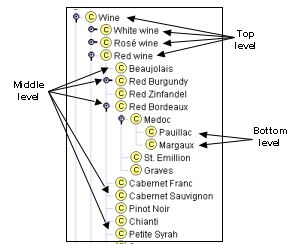
\includegraphics[scale=0.75]{figures/classhierarchical.jpg}
	\caption{Example class hierarchy from an example with wine.\cite{website:standford}}
	\label{fig:example_classhierachy}
\end{figure}

It is not enough with dividing only the classes to get the answers that is pointed out in the first step, it is also necessary to define properties to the classes. For each property we define, we have to define which class the property contain. The subclasses of a class inherits the properties from that class and a property should also be attached to the most general class that can have that property.

Each property also have to be defined a type. Examples of different types can be: string, number, boolean, enumerated and instance. String is a text string. Number can be float or integer. The boolean type is just a true/false value or it can be 1/0, where 1 is true and 0 is false. Enumerated is a list of allowed values. Instance allow to definition of relationship between individuals.

The last step is to create the instances. To define an individual instance of a class, there are three steps:
\begin{enumerate}
	\item Choosing a class
	\item Creating an instance of the chosen class
	\item Filling in the properties for the chosen instance.
\end{enumerate}
\cite{website:standford}